\chapter{Datasets and running conditions}
\label{chap:prod:data}

The data used for this measurement were collected at the very beginning of 
\runtwo\ of the \ac{LHC}, during a special 15-day `early measurements' period.
The number of bunches in the accelerator was gradually increased from 50 at the 
beginning to 482 bunches at the end of the period, with the number colliding at 
IP8 increasing from 36 to 397 bunches.
In addition, the minimum bunch spacing was set to \SI{50}{\nano\second}, as in 
\runone, rather than the nominal \runtwo\ spacing of \SI{25}{\nano\second}.
These steps were taken primarily for machine safety, as the \ac{LHC} began 
operating at a new centre-of-mass energy, \sqrtseq{13}, never before seen at a 
particle collider.

Despite taking precautions, the machine suffered several technical problems 
during this period, and so a significant amount of time allocated for `physics 
running' was lost to recovery.
At \lhcb, each \ac{LHC} fill is indexed with a number, and this measurement 
uses fills 3976, 3981, 3988, 3992, and 3996.
The combination of these fills corresponds to around \SI{32}{\hour} of 
collisions.
Other fills taken during the early measurements period were excluded from the 
analysis due to them either being of a short length of time, usually 
corresponding to unstable beam conditions, or because one or more \lhcb\ 
sub-detector was found to be operating incorrectly during data-taking.

The combined dataset used for the measurement corresponds to an integrated 
luminosity, defined in \cref{eqn:prod:introduction:integrated_lumi}, of
\begin{equation}
  \intlumi = \SI{\xsectotlumi}{\per\pico\barn}.
  \label{eqn:prod:xsectotlumi}
\end{equation}
The measurement of this quantity will be described in 
\cref{chap:prod:data:lumi}.
For reference, the total integrated luminosity collected in \runone\ at \lhcb\ 
was \SI{3}{\per\femto\barn}, 600 times more, whilst that for the \sqrtseq{7}\ 
\lhcb\ open charm production measurement was \SI{15}{\per\nb}, 300 times less.
All data were taken with the \lhcb\ dipole magnet in the `down' polarity, and 
were processed via the Turbo stream data flow, as described in 
\cref{chap:intro:lhcb:detector}.
A matching set of simulated \ac{MC} events is also used in the analysis, which 
is described in \cref{chap:prod:data:mc}.
The selection of events and charm candidates, both in the trigger and offline, 
will be described in \cref{chap:prod:sel}.

\section{Luminosity determination}
\label{chap:prod:data:lumi}

The luminosity was measured in a dedicated analysis as part of the general 
\lhcb\ early measurements campaign.
The luminosity is used as input not only for the open charm production analysis 
discussed here, but also in the measurements of \PJpsi and \PB hadron 
production~\cite{LHCb-PAPER-2015-037,LHCb-PAPER-2016-031}, which were also part 
of that campaign.
This \namecref{chap:prod:data:lumi} shall briefly describe how the luminosity 
was measured, as it is a key component to the measurement and contributes 
significantly to the final uncertainty on it.

The instantaneous luminosity is defined in \cref{eqn:intro:lhc:inst_lumi}, and 
can be re-formulated more succinctly as
\begin{equation}
  \lumi = N_{\text{p}}^{2}\revfreq\Omega,
  \label{eqn:prod:data:lumi}
\end{equation}
where $\Omega$ encapsulates the overlapping bunch densities.
If each bunch, 1 and 2, has particle density distributions $\rho_{1}(x, y, z, 
t)$ and $\rho_{2}(x, y, z, t)$, the overlap can be expressed as
\begin{equation}
  \Omega \propto \int \rho_{1}(x, y, z, t)\rho_{2}(x, y, z, t)
                      \dif{x}\dif{y}\dif{z}\dif{t}.
  \label{eqn:prod:data:lumi:profile}
\end{equation}
In general, this quantity is different at each \acl{LHCIP}, and so each 
experiment performs measurements of it.
At \lhcb, two methods have been used to measure the bunch 
profiles~\cite{LHCb-PAPER-2014-047}.
% TODO ok, but what is done with the scan data?
The first is the \ac{VDM} scan, where the beams are scanned across each other 
in fine $x$ and $y$ steps to measure the transverse profile.
This technique is also used in the \atlas, \cms, and \alice\ experiments, where 
it is the only available method for measuring the bunch profiles.
The \ac{VDM} scan measurement assumes that the profiles in $x$ and $y$ are 
factorisable, such as being two independent Gaussian distributions.
The high precision of the \lhcb\ \velo\ sub-detector allows for the second 
method: the \ac{BGI}.
This method uses gas injected into the \ac{LHC} vacuum inside the \velo\ 
sub-detector to create `beam-gas' interactions.
The vertices of these interactions can be reconstructed using track segments 
formed in the \velo and the distribution of vertices gives the 
three-dimensional beam profile, shown in \cref{fig:prod:data:lumi:bgi_fits}.

As the \ac{VDM} and \ac{BGI} methods are independent, they serve as 
cross-checks of one another and can be combined in an average if they are 
compatible.
They were both used in an analysis to measure the \runone\ integrated 
luminosity where a relative uncertainty on the combination of 
\SI{1.16}{\percent} was achieved, the highest precision on a luminosity 
measurement at an \ac{LHC} experiment~\cite{LHCb-PAPER-2014-047}.
For the early measurements campaign, only the data for the \ac{BGI} measurement 
was available, and a precision of \SI{3.8}{\percent} was reached.

Both the \ac{VDM} and the \ac{BGI} methods require special \ac{LHC} running 
conditions.
The data for the luminosity analysis is collected during dedicated fills and is 
not used for physics analyses.
The absolute luminosity is then determined only for these fills, and so it is 
necessary to translate this to a luminosity measurement for the fills used for 
physics data.
This is done by choosing a set of processes whose rates are proportional to the 
visible \pp\ interaction rate, and using the constant of proportionality as 
measured during the absolute luminosity measurement.
These `luminosity counters', such as the number of tracks reconstructed in the 
\velo, the energy deposited in the hadronic calorimeter, or even the fraction 
of beam-beam crossings where no activity was seen in the detector, are stored 
alongside the data during physics running.
The total luminosity for a dataset used in an analysis is then determined by 
integrating the values from a counter and dividing it by the corresponding 
absolute luminosity calibration constant.

\begin{figure}
  \centering
  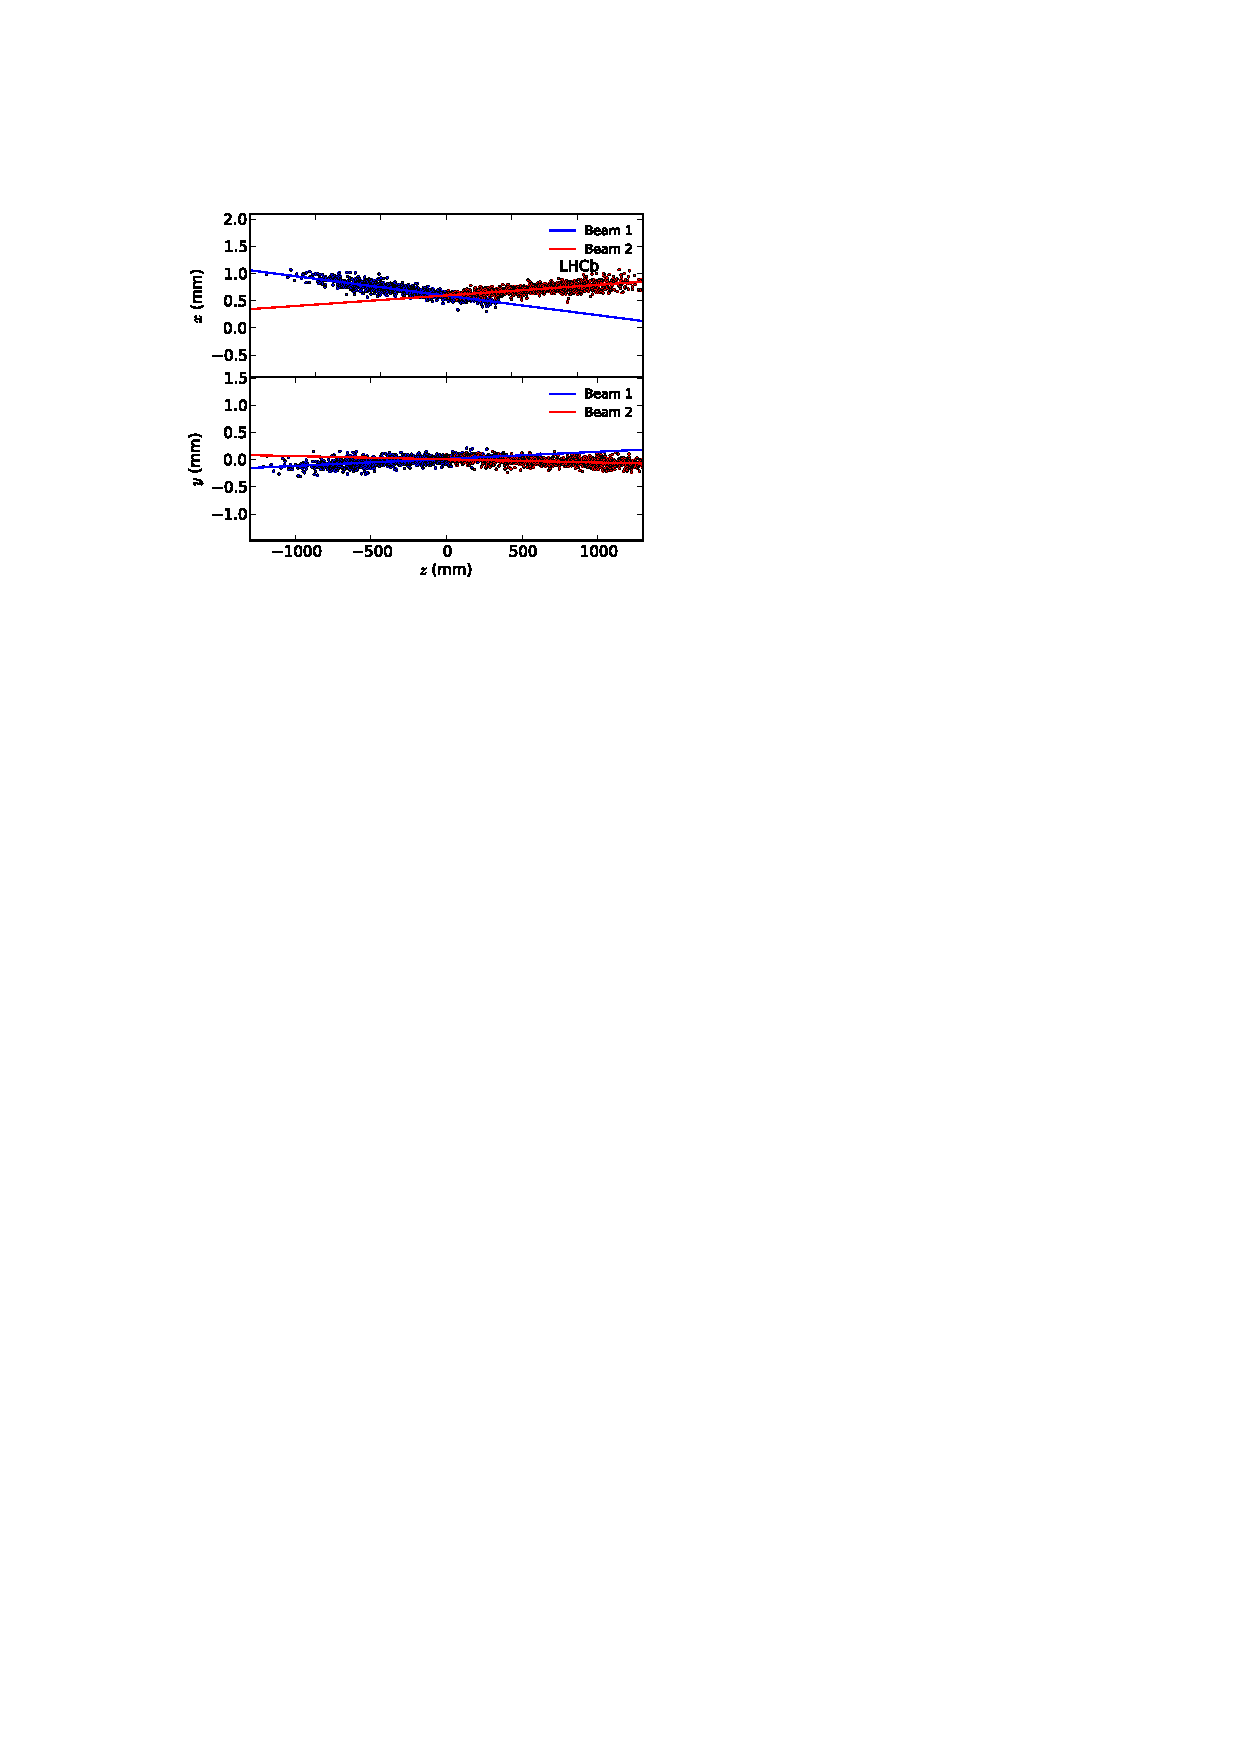
\includegraphics[width=\textwidth]{production/bgi_fits}
  \caption{%
    Projections of fits to beam-gas interaction vertices used as part of a 
    \acl{BGI} luminosity measurement~\cite{LHCb-PAPER-2014-047}.
    The data shown were used for the \ac{BGI} measurement at \sqrtseq{8} in 
    2012.
    For illustrative purposes only the first \num{1000} interaction vertices 
    are shown per beam.
  }
  \label{fig:prod:data:lumi:bgi_fits}
\end{figure}

\section{Simulated data samples}
\label{chap:prod:data:mc}

If an event is not selected by the trigger, it lost for analysis.
In order to have access to information before this stage, simulated \acf{MC} 
samples are generated.

Proton-proton collisions are generated by the \pythia\ 8 program, which 
simulates the parton interactions, quark and gluon fragmentation, and resulting 
hadronisation and creation of other particles, such as leptons.
The behaviour of the hadrons is simulated by the \evtgen\ program, which models 
phenomena such as branching fractions, neutral meson mixing, \CP\ violation, 
decay amplitude models, and decay times.
Simulated samples for a specific decay are generated by running \pythia\ in 
`minimum bias mode', where proton-proton collisions are generated until the 
head of the decay is created somewhere in the set of particles produced, and 
then this head particle is forced to decay to the final state under study by 
\evtgen~\cite{Clemencic:2011zza}.
The behaviour of the other particles generated in the event is also controlled 
by \evtgen, but is not forced to any particular state.
The total simulation is configured to model the beam parameters relating to the 
`real data' the \ac{MC} is to be used with~\cite{Belyaev:1322400}.
After \evtgen, the particles are propagated through a simulation of the entire 
detector using the \geant\ 4 program, where interactions with the detector are 
recorded as `\ac{MC} hits'.
These \ac{MC} hits are converted into a format mimicking the electrical 
response of the real detector through an \lhcb-specific emulation, and the 
response is processed through the trigger and reconstruction software in an 
identical manner to real data.

This analysis uses simulated samples of \DstToDzpi\ with \DzToKpi, \DpToKpipi, 
and \DspToKKpi\ decays.
The \DstToDzpi\ sample is sufficient for studying both \DstToDzpi\ and 
(untagged) \DzToKpi efficiencies, as the effect of the soft pion is 
parameterised in \PDzero\ \pT\ and \rapidity, which this measurement is also 
parameterised in.
In addition, the \DspToKKpi\ sample is sufficient for studying \DspTophipi\ 
decays, given that the kaon pair is required to be within the same mass window 
applied to the data.
For each decay mode, samples of \num{2.5} millions events are generated, with 
an additional \num{1} million events generated where the decay head is required 
to have $\pT > \SI{10}{\GeVc}$.
To save computing resources, the decays are required to be within the \lhcb\ 
geometric acceptance after \evtgen\ has run.
This requirement imposes all charged final state particles have a positive $z$ 
component of their three-momentum and that they satisfy
\begin{equation}
  10 < \theta < \SI{400}{\milli\radian},
  \label{eqn:prod:data:lhcb_acceptance}
\end{equation}
where $\theta$ is the polar angle.
As this cut is not \SI{100}{\percent} efficient in some \pTy\ bins, its 
efficiency must be assessed, as described in \cref{chap:prod:effs:acc}, and so 
dedicated, generator-only datasets are also produced.
These data are not processed beyond the \evtgen\ step.

The simulated data is processed in such a way that reconstructed objects can be 
associated to the \ac{MC} objects that created them.
For charged, stable particles reconstructed via tracks, a particle is 
associated to an \ac{MC} particle if at least \SI{70}{\percent} of the hits 
comprising the associated track were deposited by the \ac{MC} particle in 
question.
The process of assigning \ac{MC} objects to reconstructed objects is referred 
to as \emph{truth matching}.
Tracks are classified as \emph{ghost} tracks if there are no \ac{MC} particles 
that can be associated to them.
Vertices can then be assigned categories based on the associations of their 
input tracks.
A signal vertex is one in which all inputs are associated to \ac{MC} particles, all inputs have been assigned a particle identity equal to that of its associated \ac{MC} particle, all inputs have been associated with \ac{MC} particles which come from the same true \ac{MC} parent, and the identity of the \ac{MC} parent matches that assigned to the vertex.
Any deviation from these requirements results in the vertex being assigned a particular \emph{background category}, dependent on the nature of the deviations~\cite{Gligorov:1035682}.
For example, if at least one track is a ghost, the vertex is classified as a ghost, and if at least one track is associated to an \ac{MC} particle with a different \ac{PID}, the vertex is classified as a misidentification.
In the case of a vertex than can be associated to an \ac{MC} particle, the 
vertex can be further classified as prompt or secondary based on the true 
lifetime of the \ac{MC} particle.
For this analysis, a vertex is classified as secondary if any particle in the 
ancestry of the associated \ac{MC} particle has a lifetime greater than 
\SI{0.1}{\femto\second}.\footnotemark
In what follows, the \ac{MC} data has been filtered such that only 
truth-matched, prompt charm hadron candidates remain, unless stated otherwise.

\footnotetext{%
  The order of magnitude of the lifetimes of the ground-state charm and beauty 
  hadrons is between $0.1$ and \SI{1}{\pico\second}.
}

\section{Crossing angle correction}
\label{chap:prod:data:crossing_angle}

Due to the non-zero crossing angles of the two proton beams provided by the 
\ac{LHC}, the \pp\ collision frame is boosted with respect to the laboratory 
frame.
As this measurement is made in bins of charm hadron transverse momentum and 
rapidity measured in the \pp\ collision rest frame, a correction must be 
applied to the \pT\ and \rapidity\ measured in the laboratory frame.

Two crossing angles are defined per beam: $\theta_{h}$ is the angle made with 
the $z$ axis in the horizontal $xz$ plane, and $\theta_{v}$ is the angle made 
with the $z$ axis in the vertical $yz$ plane.
With $\theta_{h} = 0$ and $\theta_{v} = 0$, the beams have the four-momentum
\begin{equation}
  p_{z+}^{\mu} = \begin{pmatrix}\Ebeam\\0\\0\\\pbeam\end{pmatrix}
    \quad\text{and}\quad
  p_{z-}^{\mu} = \begin{pmatrix}\Ebeam\\0\\0\\-\pbeam\end{pmatrix},
\end{equation}
where $z\pm$ marks the beam moving with increasing or decreasing $z$, \Ebeam\ 
is the nominal beam energy of $\sqrts/2 = \SI{6.5}{\TeV}$, and \pbeam\ is the 
beam momentum as $\pbeam^{2} = \Ebeam^{2} - m_{\text{Proton}}^{2}$.
With non-zero crossing angles, the beam four-vectors become
\begin{align}
  p_{z+}^{\mu} &= \begin{pmatrix}
    \Ebeam\\
    \pbeam\sin{\theta_{h,+}}\\
    \pbeam\sin{\theta_{v,+}}\\
    \pbeam\sqrt{1 - \sin^{2}{\theta_{h,+}} - \sin^{2}{\theta_{v,+}}}
  \end{pmatrix}\quad\text{and}\nonumber\\
  p_{z-}^{\mu} &= \begin{pmatrix}
    \Ebeam\\
    -\pbeam\sin{\theta_{h,-}}\\
    -\pbeam\sin{\theta_{v,-}}\\
    -\pbeam\sqrt{1 - \sin^{2}{\theta_{h,-}} - \sin^{2}{\theta_{v,-}}}
  \end{pmatrix},
\end{align}
where $\theta_{h,\pm}$ and $\theta_{v,\pm}$ are defined to allow for 
asymmetrical crossing angles between the two beams.
The centre-of-mass four vector $\ptot_{\text{CoM}}^{\mu}$ is then the sum of 
$p_{z+}^{\mu}$ and $p_{z-}^{\mu}$.

Charm hadron candidates in both the real data and the \ac{MC} are boosted into 
the centre-of-mass rest frame, and the system is then rotated to make the 
boosted beam $z$ axis coincident with that in the laboratory frame.
The transverse momentum and rapidity are then recomputed and recorded.
Example \pT\ and \rapidity\ distributions as measured in the laboratory and 
\pp\ centre-of-mass frames are given for the simulated \DstToDzpi\ dataset in 
\cref{fig:prod:data:com_boost}.
Whenever charm hadron \pT\ or \rapidity\ are mentioned, it is the \pp\ rest 
frame quantities that are used, unless stated otherwise.

In the data sample used, the only non-zero crossing angle was in the $xz$ plane 
and this was symmetric between the two beams.
The crossing angle values were $\theta_{h,+} = -\theta_{h,-} = 
\SI{790}{\micro\radian}$ and $\theta_{v,+} = -\theta_{v,-} = 
\SI{0}{\micro\radian}$.
These values are used in the beam parameterisation in the \ac{MC} data.

\begin{figure}
  \begin{subfigure}[b]{0.5\textwidth}
    \centering
    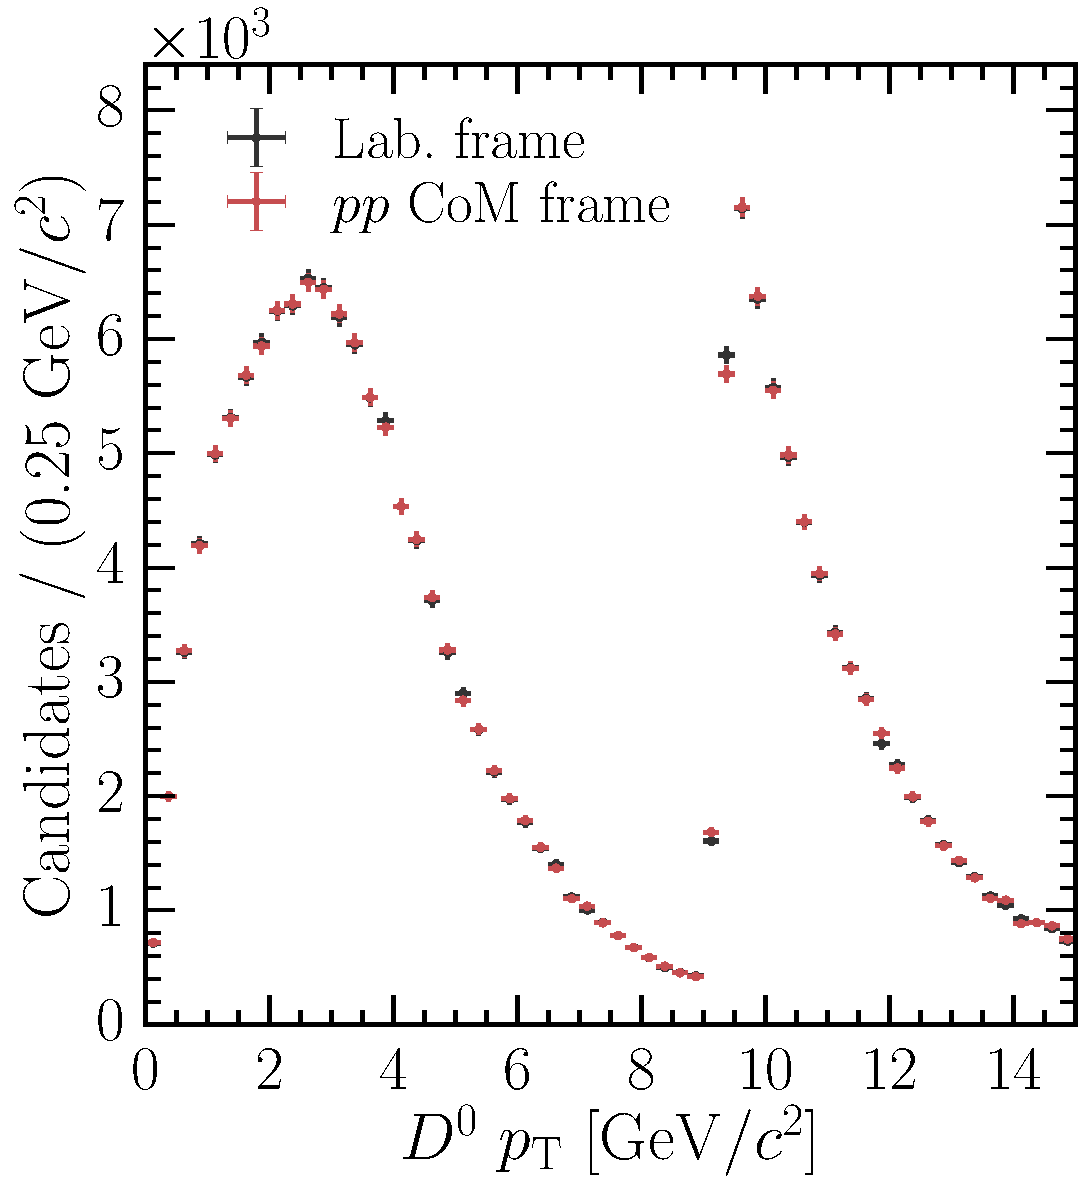
\includegraphics[width=\textwidth]{production/data/D0ToKpi_MC_PT}
    \caption{\pT}
    \label{fig:prod:data:com_boost:pt}
  \end{subfigure}
  \begin{subfigure}[b]{0.5\textwidth}
    \centering
    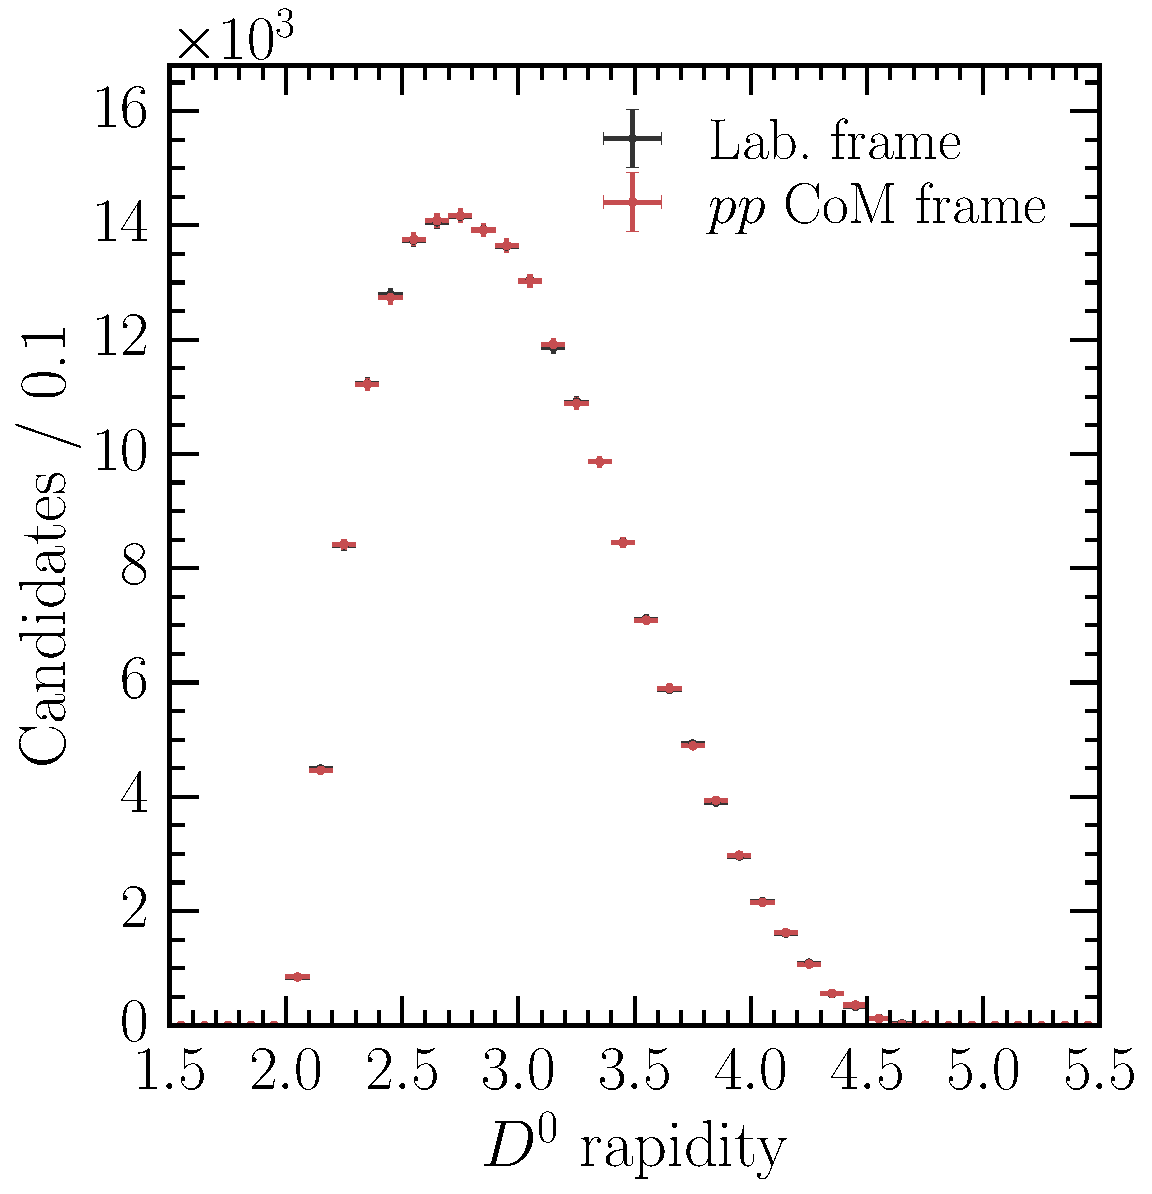
\includegraphics[width=\textwidth]{production/data/D0ToKpi_MC_Y}
    \caption{\rapidity}
    \label{fig:prod:data:com_boost:y}
  \end{subfigure}
  \caption{%
    Distributions of \PDzero\ \pT~(\subref*{fig:prod:data:com_boost:pt}) and 
    \rapidity~(\subref*{fig:prod:data:com_boost:y}) as measured in the 
    laboratory frame (black) and in the proton-proton centre-of-mass~(CoM) 
    frame (red), in the simulated \DstToDzpi, with \DzToKpi, dataset.
  }
  \label{fig:prod:data:com_boost}
\end{figure}
